\documentclass[aspectratio=169, 10pt]{beamer}
\usepackage{beamer_theme_cienciadados2026}
\usepackage{graphicx}

\title[Aula 01 - História e Introdução]{Ciência dos Dados I: Análise Exploratória}
\subtitle{Aula 01: Introdução e História da Computação à Ciência dos Dados}
\author{Prof. Dr. Ney Lemke}
\institute{UNESP -- Instituto de Biociências de Botucatu \\ Curso de Física Médica}
\date{Versão 2026}

\begin{document}

% Slide 1: Título
\frame{\titlepage}

% Slide 2: Sumário
\begin{frame}{Sumário da Aula}
  \tableofcontents
\end{frame}

% ----------------------------------------------------
\section{Introdução e a Metáfora dos Dados}
% ----------------------------------------------------

\begin{frame}{O Catálogo de Leporello em \textit{Don Giovanni}}
  \begin{columns}
    \begin{column}{0.55\textwidth}
      Na ópera de Mozart e Da Ponte (1787), o servo Leporello apresenta o registro metódico das conquistas de Don Giovanni:
      \begin{quote}
        \small
        \textit{"Madamina, il catalogo è questo \\
        delle belle, che amò il padron mio; \\
        un catalogo egli è, che ho fatt'io. \\
        In Italia seicento e quaranta, \\
        in Almagna duecento e trentuna, \\
        cento in Francia, in Turchia novantuna, \\
        ma in Ispagna son già mille e tre!"}
      \end{quote}
    \end{column}
    \begin{column}{0.42\textwidth}
      \begin{block}{O que é este Catálogo?}
        \begin{itemize}
          \item \textbf{Coleta sistemática} de observações.
          \item \textbf{Estratificação} por categorias (geografia, estrato social, idade).
          \item \textbf{Agregação quantitativa}: uma autêntica prefiguração da análise exploratória!
        \end{itemize}
      \end{block}
    \end{column}
  \end{columns}
\end{frame}

\begin{frame}{O que é Ciência de Dados?}
  \begin{columns}
    \begin{column}{0.55\textwidth}
      \textbf{Definição}: Disciplina que combina métodos científicos, processos algorítmicos e inteligência quantitativa para extrair conhecimento de dados ruidosos.
      \begin{itemize}
        \item \textbf{Computação e Engenharia}: manipulação eficiente, código limpo, reprodutibilidade.
        \item \textbf{Matemática e Estatística}: inferência, distribuições, modelagem e incerteza.
        \item \textbf{Conhecimento de Domínio}: Física Médica, Biologia, Saúde e Biofísica.
      \end{itemize}
    \end{column}
    \begin{column}{0.42\textwidth}
      \begin{block}{John Tukey (1962)}
        \textit{"A análise exploratória de dados é uma atitude, uma flexibilidade e uma disposição para buscar coisas além do que esperávamos encontrar."}
      \end{block}
      \begin{exampleblock}{O Papel da EDA}
        Compreender a estrutura dos dados antes de qualquer hipótese ou modelo preditivo.
      \end{exampleblock}
    \end{column}
  \end{columns}
\end{frame}

% ----------------------------------------------------
\section{Primórdios da Coleta e Registro de Dados}
% ----------------------------------------------------

\begin{frame}{As Cheias do Nilo: Previsão e Séries Temporais Antigas}
  \begin{columns}
    \begin{column}{0.5\textwidth}
      \begin{itemize}
        \item A civilização egípcia dependia criticamente do regime anual de cheias do Rio Nilo para a agricultura.
        \item A narrativa bíblica de José no Egito ilustra a gestão baseada em previsão de safras e armazenamento estratégico de estoques.
        \item \textbf{Nilômetros}: marcos de pedra que registravam historicamente os níveis do rio -- uma das primeiras bases de dados de séries temporais da humanidade.
      \end{itemize}
    \end{column}
    \begin{column}{0.48\textwidth}
      \centering
      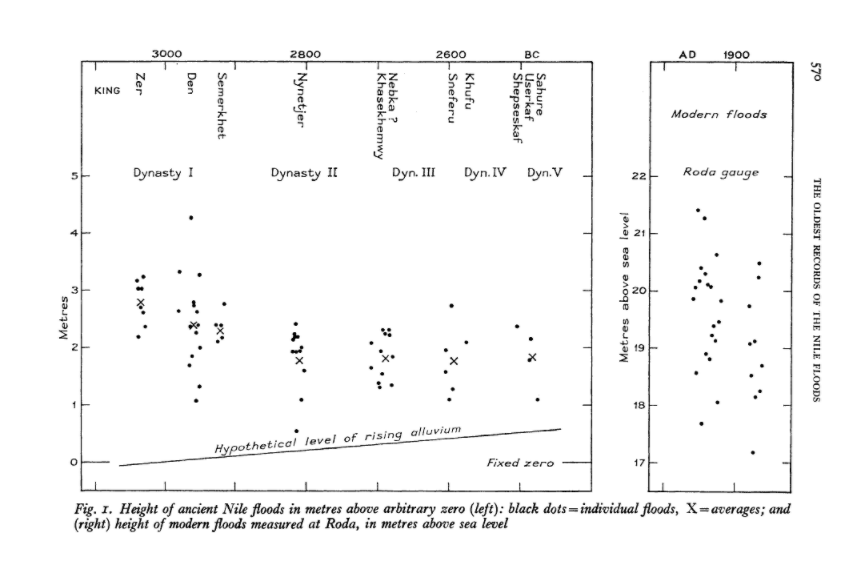
\includegraphics[width=\linewidth, height=0.72\textheight, keepaspectratio]{enchentes.png}
      \par\vspace{0.2em}{\scriptsize \textit{Registros e dinâmica histórica de inundações.}}
    \end{column}
  \end{columns}
\end{frame}

\begin{frame}{A Tableta Suméria: Os Primeiros Registros Contábeis}
  \begin{columns}
    \begin{column}{0.5\textwidth}
      \begin{itemize}
        \item Na Mesopotâmia (c. 3200 a.C.), a escrita cuneiforme em argila não nasceu para a poesia, mas para a \textbf{contabilidade}.
        \item Registros detalhados de sacas de cevada, rebanhos, impostos e transações comerciais.
        \item O dado enquanto prova documental e base para a tomada de decisões administrativas do Estado sumério.
      \end{itemize}
    \end{column}
    \begin{column}{0.48\textwidth}
      \centering
      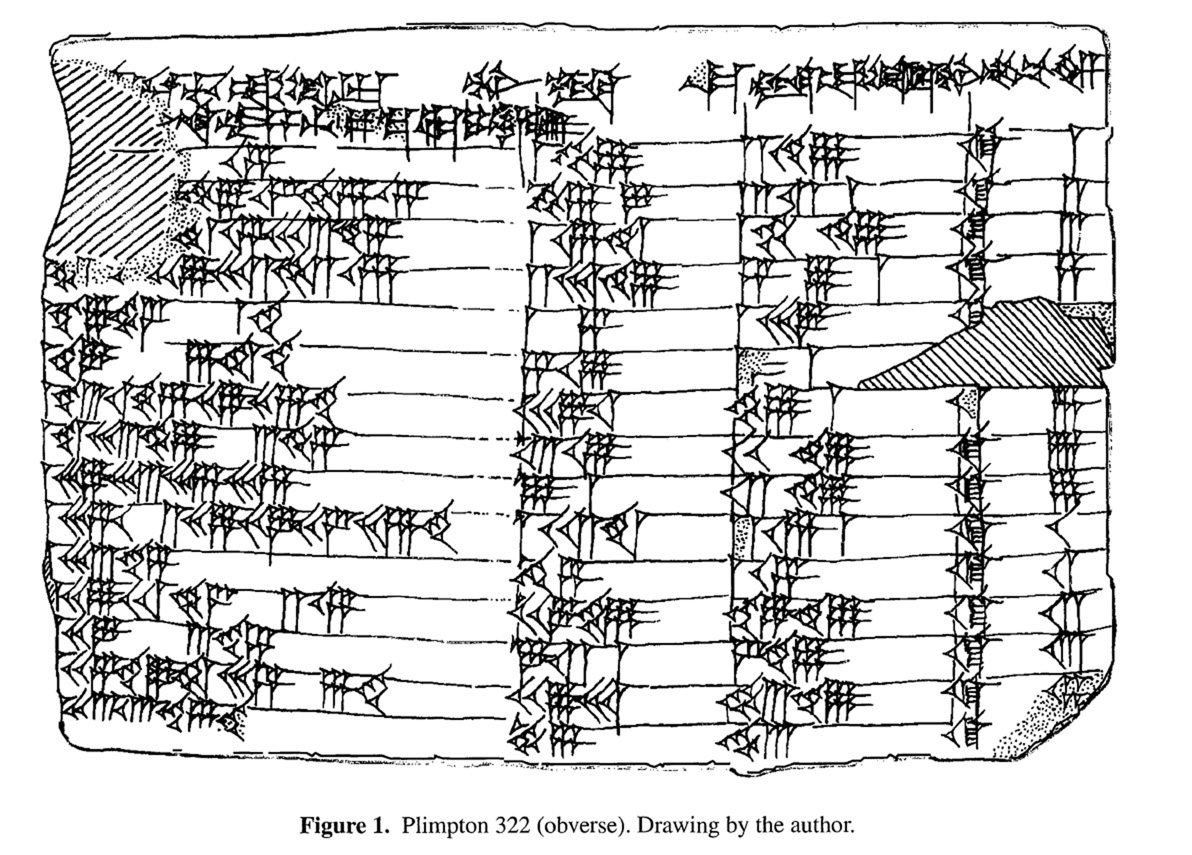
\includegraphics[width=\linewidth, height=0.72\textheight, keepaspectratio]{tabletaSumeria.png}
      \par\vspace{0.2em}{\scriptsize \textit{Tableta suméria em argila com registros contábeis.}}
    \end{column}
  \end{columns}
\end{frame}

% ----------------------------------------------------
\section{Instrumentos de Cálculo e Análise Pré-Eletrônicos}
% ----------------------------------------------------

\begin{frame}{O Ábaco: A Computação Mecânica}
  \begin{columns}
    \begin{column}{0.5\textwidth}
      \begin{itemize}
        \item Utilizado na Babilônia, China, Grécia e Roma antiga.
        \item Representação posicional de números e realização rápida de operações aritméticas fundamentais.
        \item A primeira grande abstração: separar o \textbf{dado bruto} da \textbf{operação computacional} realizada sobre ele.
      \end{itemize}
    \end{column}
    \begin{column}{0.48\textwidth}
      \centering
      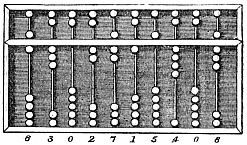
\includegraphics[width=\linewidth, height=0.72\textheight, keepaspectratio]{Abacus_6.png}
      \par\vspace{0.2em}{\scriptsize \textit{Ábaco tradicional: ferramenta de cálculo aritmético.}}
    \end{column}
  \end{columns}
\end{frame}

\begin{frame}{O Astrolábio: Instrumento Astronômico e Analógico}
  \begin{columns}
    \begin{column}{0.5\textwidth}
      \begin{itemize}
        \item Desenvolvido na Antiguidade helenística e aperfeiçoado no Mundo Islâmico medieval.
        \item Computador analógico bidimensional para cálculo da posição do Sol, estrelas e navegação.
        \item Transformação de coordenadas esféricas celestes para o plano (projeção estereográfica).
      \end{itemize}
    \end{column}
    \begin{column}{0.48\textwidth}
      \centering
      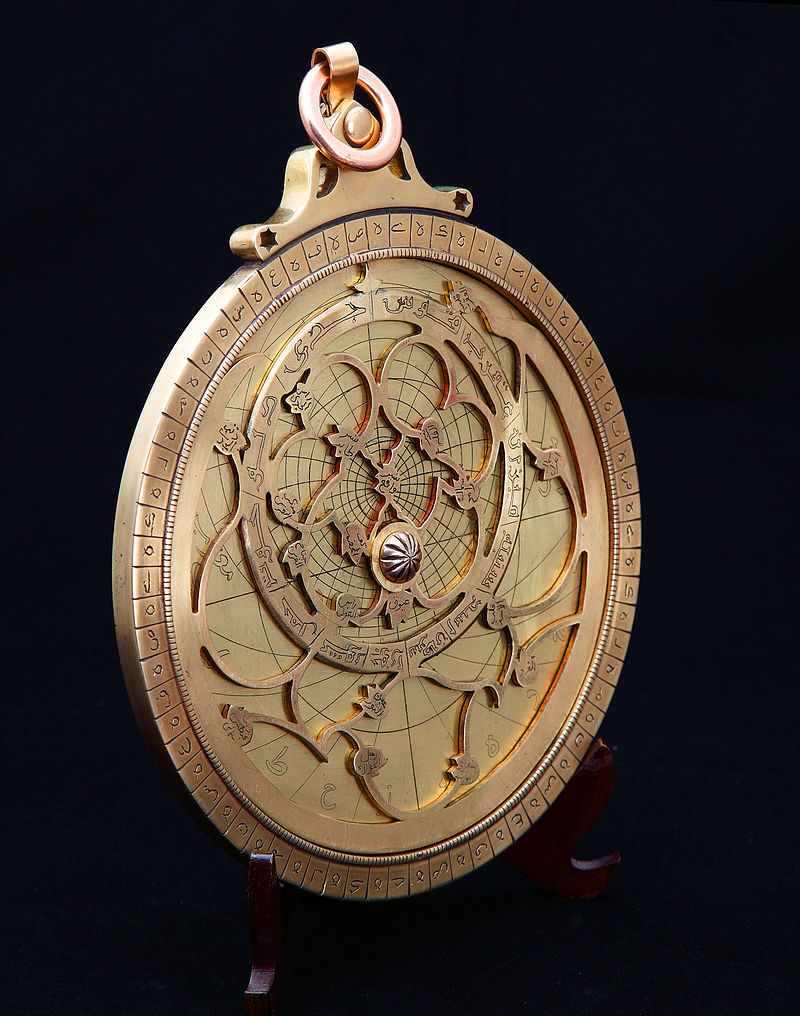
\includegraphics[width=\linewidth, height=0.72\textheight, keepaspectratio]{800px-Iranian_Astrolabe_14.jpg}
      \par\vspace{0.2em}{\scriptsize \textit{Astrolábio persa do século XVIII.}}
    \end{column}
  \end{columns}
\end{frame}

\begin{frame}{Tycho Brahe, Kepler e a Astronomia Guiada por Dados}
  \begin{columns}
    \begin{column}{0.52\textwidth}
      \begin{itemize}
        \item \textbf{Tycho Brahe (1546--1601)}: Realizou décadas de medições astronômicas com precisão sem precedentes, sem o uso de telescópios.
        \item \textbf{Johannes Kepler (1571--1630)}: Analisou meticulosamente os dados tabulares de Marte herdados de Tycho.
        \item \textbf{Conclusão}: Ao confiar nos dados empíricos em vez de dogmas circulares, Kepler deduziu que as órbitas planetárias são \textbf{elipses}!
      \end{itemize}
    \end{column}
    \begin{column}{0.46\textwidth}
      \centering
      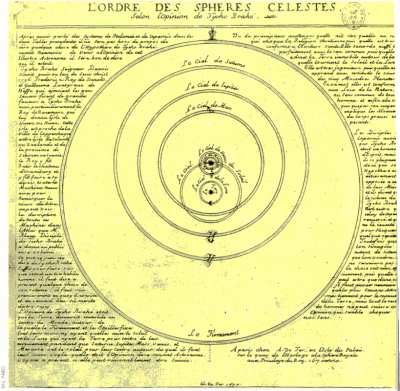
\includegraphics[width=\linewidth, height=0.72\textheight, keepaspectratio]{universo_titonico.png}
      \par\vspace{0.2em}{\scriptsize \textit{O sistema cosmológico tichônico.}}
    \end{column}
  \end{columns}
\end{frame}

\begin{frame}{A Régua de Cálculo: Três Séculos de Engenharia}
  \begin{columns}
    \begin{column}{0.5\textwidth}
      \begin{itemize}
        \item Inventada por William Oughtred no século XVII baseada nos logaritmos de John Napier.
        \item Converte multiplicações e divisões em adições e subtrações visuais de comprimentos logarítmicos.
        \item Foi o instrumento computacional de cientistas e engenheiros até o Projeto Apollo na década de 1960!
      \end{itemize}
    \end{column}
    \begin{column}{0.48\textwidth}
      \centering
      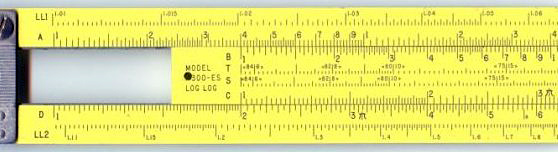
\includegraphics[width=\linewidth, height=0.72\textheight, keepaspectratio]{Pocket_slide_rule.jpg}
      \par\vspace{0.2em}{\scriptsize \textit{Régua de cálculo portátil.}}
    \end{column}
  \end{columns}
\end{frame}

\begin{frame}{Gregor Mendel: A Estatística nas Origens da Genética}
  \begin{columns}
    \begin{column}{0.5\textwidth}
      \begin{itemize}
        \item O monge agostiniano Gregor Mendel (1822--1884) cultivou cerca de 28.000 pés de ervilha.
        \item Contagem sistemática de traços fenotípicos (amarelo/verde, liso/rugoso).
        \item A proporção matemática observada de $3:1$ permitiu inferir a existência de fatores hereditários discretos (genes) muito antes do conhecimento molecular do DNA!
      \end{itemize}
    \end{column}
    \begin{column}{0.48\textwidth}
      \centering
      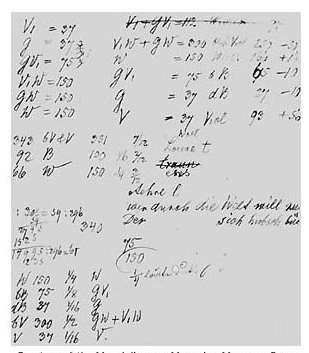
\includegraphics[width=\linewidth, height=0.72\textheight, keepaspectratio]{mendel.png}
      \par\vspace{0.2em}{\scriptsize \textit{Gregor Mendel e os dados empíricos de segregação.}}
    \end{column}
  \end{columns}
\end{frame}

% ----------------------------------------------------
\section{O Nascimento da Computação Moderna (1940--1950)}
% ----------------------------------------------------

\begin{frame}{Alan Turing e os Fundamentos da Computabilidade}
  \begin{columns}
    \begin{column}{0.52\textwidth}
      \begin{itemize}
        \item \textbf{1936}: Artigo seminal sobre os Números Computáveis e o conceito formal da Máquina de Turing.
        \item \textbf{Segunda Guerra Mundial (Bletchley Park)}: Projeto da máquina eletromecânica \textit{Bombe} para decifrar as transmissões navais nazistas codificadas pela máquina Enigma.
        \item \textbf{1950}: O artigo \textit{"Computing Machinery and Intelligence"} e o célebre Teste de Turing.
      \end{itemize}
    \end{column}
    \begin{column}{0.46\textwidth}
      \centering
      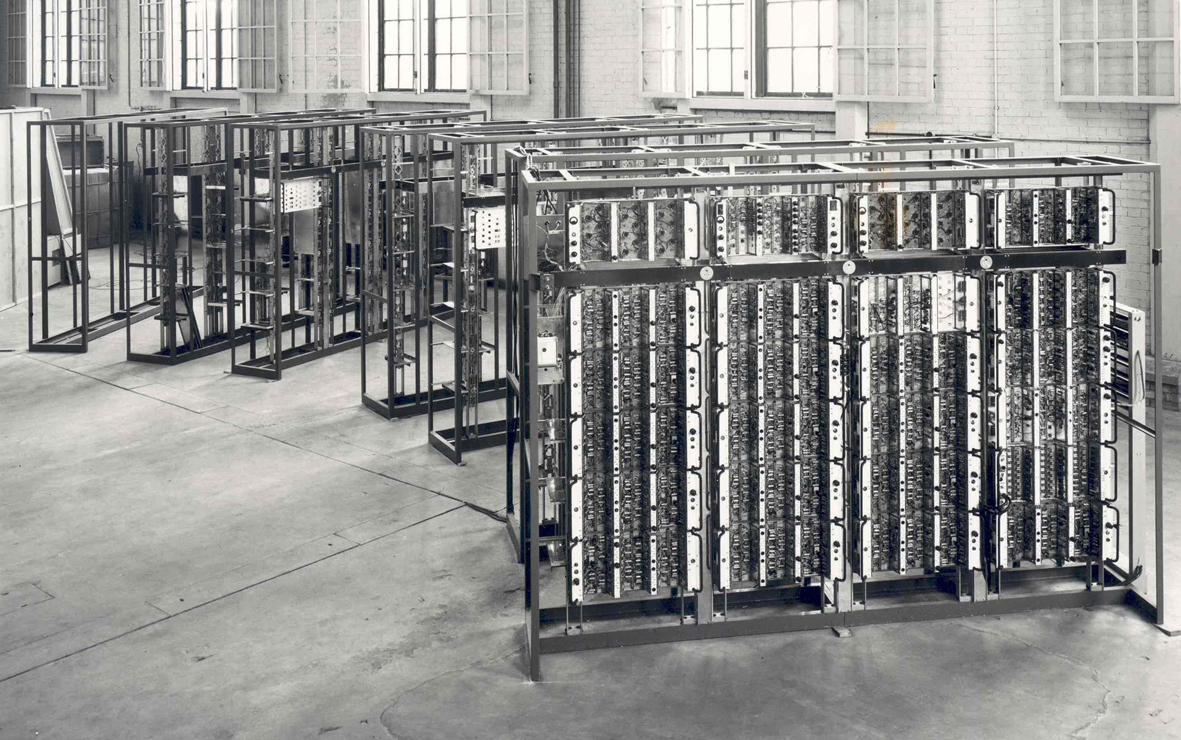
\includegraphics[width=\linewidth, height=0.72\textheight, keepaspectratio]{turing-5.jpg}
      \par\vspace{0.2em}{\scriptsize \textit{Alan Turing (1912--1954).}}
    \end{column}
  \end{columns}
\end{frame}

\begin{frame}{ENIAC e o Laboratório de Los Alamos}
  \begin{columns}
    \begin{column}{0.52\textwidth}
      \begin{itemize}
        \item \textbf{ENIAC (1945)}: Primeiro computador digital eletrônico de grande escala e de uso geral.
        \item Com mais de 17.000 válvulas termiônicas, realizava milhares de cálculos por segundo.
        \item \textbf{Física Computacional}: Utilizado por John von Neumann, Stanislaw Ulam e Nicholas Metropolis para desenvolver o \textbf{Método de Monte Carlo}, crucial para simulações nucleares.
      \end{itemize}
    \end{column}
    \begin{column}{0.46\textwidth}
      \centering
      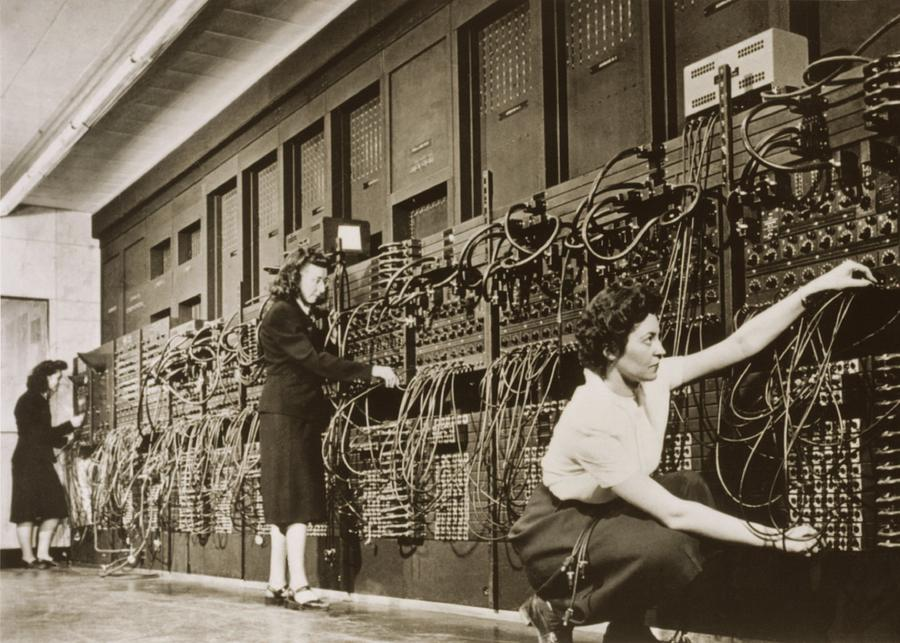
\includegraphics[width=\linewidth, height=0.72\textheight, keepaspectratio]{eniac-the-second-electronic-calculator-los-alamos-national-laboratory.jpg}
      \par\vspace{0.2em}{\scriptsize \textit{ENIAC em operação no Laboratório de Los Alamos.}}
    \end{column}
  \end{columns}
\end{frame}

% ----------------------------------------------------
\section{A Dinâmica dos Dados e seus Riscos (1960--1970)}
% ----------------------------------------------------

\begin{frame}{O Atrator de Lorenz: Caos Determinístico}
  \begin{columns}
    \begin{column}{0.52\textwidth}
      \begin{itemize}
        \item \textbf{Edward Lorenz (1963)}: Modelo simplificado de convecção atmosférica com 3 equações diferenciais acopladas.
        \item \textbf{Efeito Borboleta}: Sensibilidade extrema às condições iniciais -- pequenas variações decimais mudam completamente o desfecho futuro.
        \item Lição para o cientista de dados: modelos complexos dependem criticamente da precisão e incerteza dos dados de entrada.
      \end{itemize}
    \end{column}
    \begin{column}{0.46\textwidth}
      \centering
      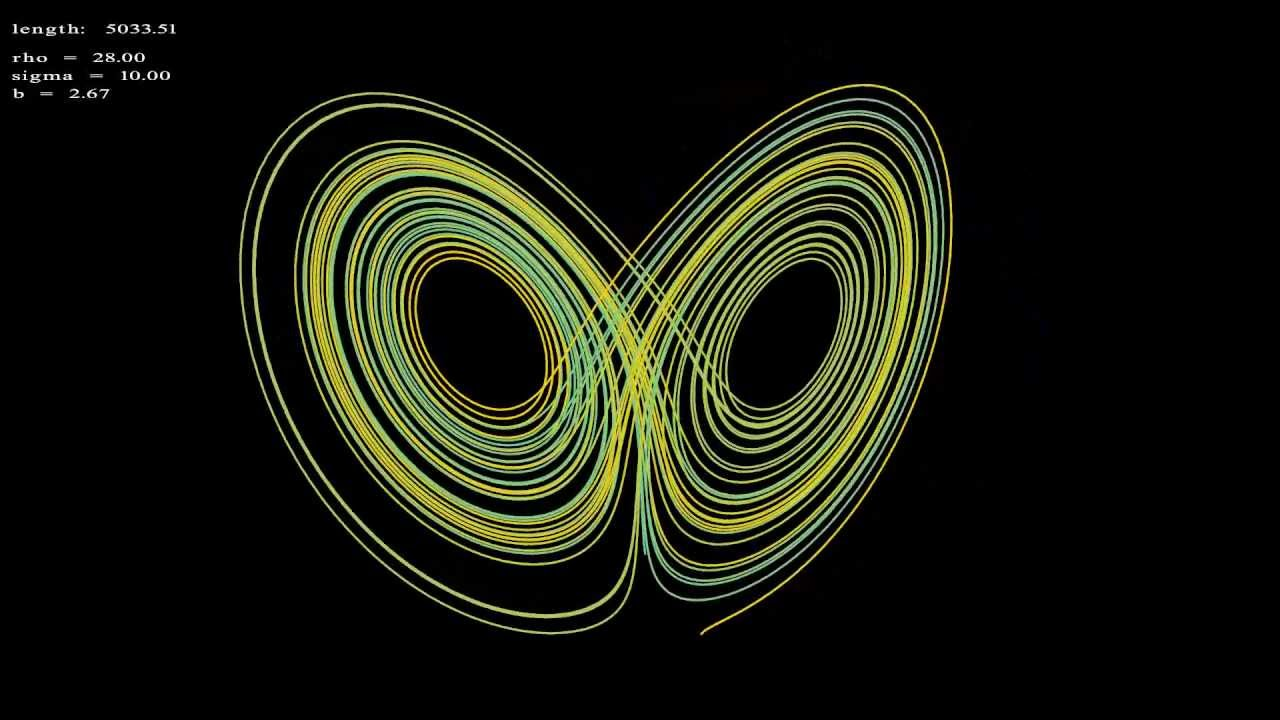
\includegraphics[width=\linewidth, height=0.72\textheight, keepaspectratio]{maxresdefault.jpg}
      \par\vspace{0.2em}{\scriptsize \textit{O atrator estranho de Lorenz no espaço de fase.}}
    \end{column}
  \end{columns}
\end{frame}

\begin{frame}{A Falácia de McNamara: Os Perigos das Métricas Cegas}
  \begin{columns}
    \begin{column}{0.52\textwidth}
      \begin{itemize}
        \item Robert McNamara (Secretário de Defesa dos EUA) aplicou gestão estritamente quantitativa na Guerra do Vietnã (\textit{"body count"}).
        \item \textbf{A Falácia}:
          \begin{enumerate}
            \item Medir tudo o que pode ser medido facilmente.
            \item Ignorar o que não pode ser facilmente quantificado.
            \item Presumir que o que não é medido não tem relevância.
            \item Dizer que o que não é medido não existe.
          \end{enumerate}
        \item \textbf{Alerta vital}: Dados sem contexto substantivo levam a catástrofes decisórias!
      \end{itemize}
    \end{column}
    \begin{column}{0.46\textwidth}
      \centering
      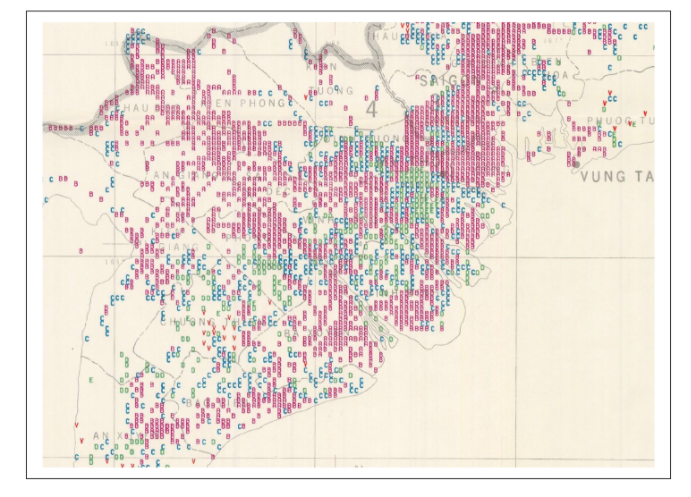
\includegraphics[width=\linewidth, height=0.72\textheight, keepaspectratio]{mcnamara.png}
      \par\vspace{0.2em}{\scriptsize \textit{Robert McNamara e a falácia das métricas isoladas.}}
    \end{column}
  \end{columns}
\end{frame}

\begin{frame}{A Revolução da HP-35 (1972)}
  \begin{columns}
    \begin{column}{0.52\textwidth}
      \begin{itemize}
        \item Primeira calculadora científica de bolso do mundo, criada pela Hewlett-Packard.
        \item Calculava funções trigonométricas e logarítmicas instantaneamente com notação polonesa reversa (RPN).
        \item Tornou a régua de cálculo obsoleta praticamente do dia para a noite nos laboratórios de física e engenharia.
      \end{itemize}
    \end{column}
    \begin{column}{0.46\textwidth}
      \centering
      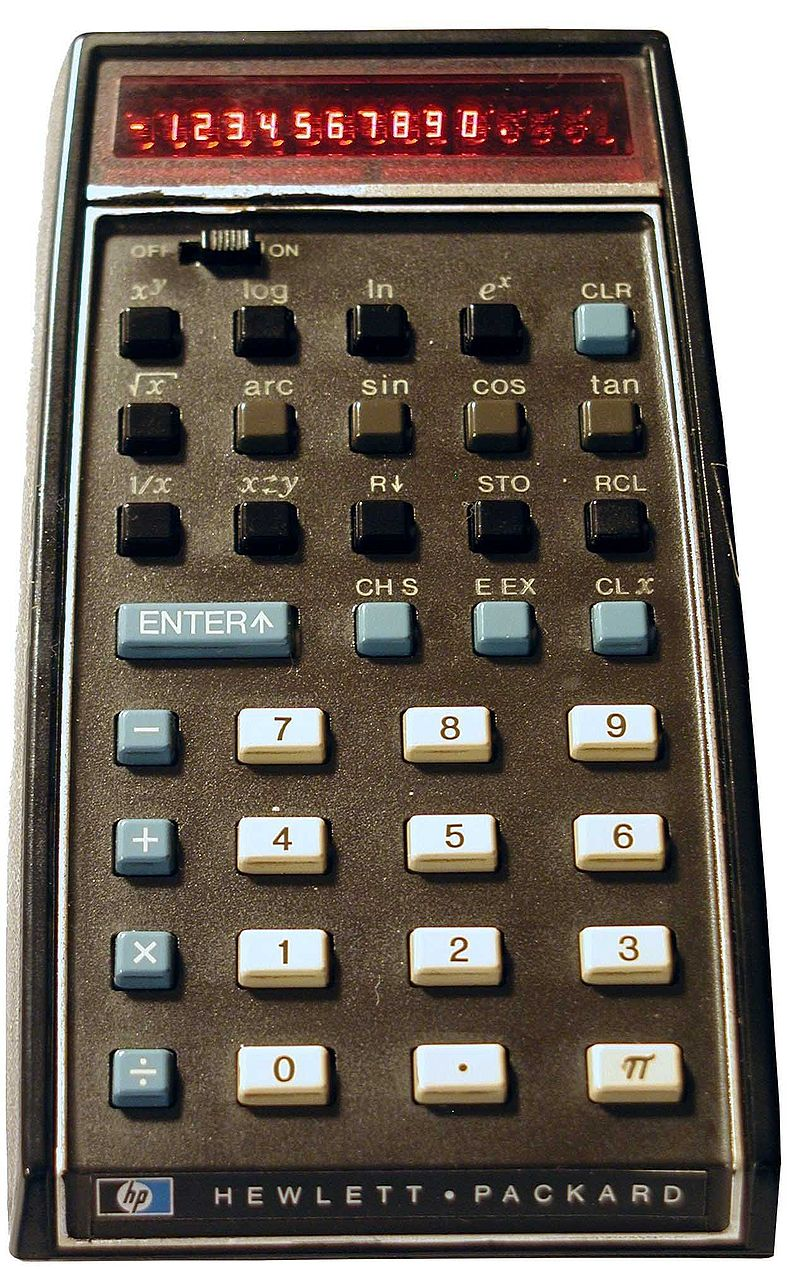
\includegraphics[width=\linewidth, height=0.72\textheight, keepaspectratio]{800px-Hp-35_1972.jpg}
      \par\vspace{0.2em}{\scriptsize \textit{Calculadora científica HP-35 (1972).}}
    \end{column}
  \end{columns}
\end{frame}

% ----------------------------------------------------
\section{Supercomputação e Redes (1980--1990)}
% ----------------------------------------------------

\begin{frame}{Seymour Cray e os Supercomputadores Vetoriais}
  \begin{columns}
    \begin{column}{0.52\textwidth}
      \begin{itemize}
        \item O \textbf{Cray-1 (1976)} introduziu arquitetura vetorial integrada de alto desempenho.
        \item Formato icônico em ferradura para minimizar o comprimento dos fios e o atraso dos sinais elétricos.
        \item Viabilizou simulações pioneiras de dinâmica molecular, meteorologia e física de plasmas.
      \end{itemize}
    \end{column}
    \begin{column}{0.46\textwidth}
      \centering
      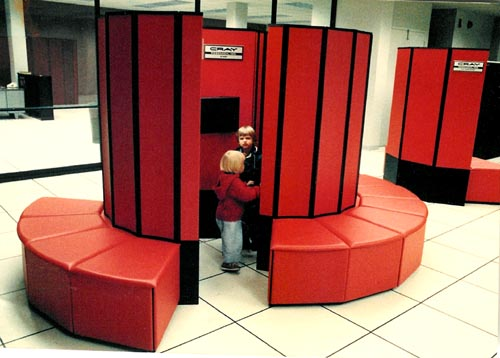
\includegraphics[width=\linewidth, height=0.72\textheight, keepaspectratio]{cray.jpg}
      \par\vspace{0.2em}{\scriptsize \textit{Supercomputador Cray-1.}}
    \end{column}
  \end{columns}
\end{frame}

% ----------------------------------------------------
\section{A Era dos Grandes Dados Biomédicos (2000--2026)}
% ----------------------------------------------------

\begin{frame}{O Projeto Genoma Humano (2001)}
  \begin{columns}
    \begin{column}{0.52\textwidth}
      \begin{itemize}
        \item Em fevereiro de 2001, a revista \textit{Nature} publica a sequência preliminar do genoma humano (3 bilhões de pares de bases).
        \item Marco histórico: a Biologia e a Física Médica transformam-se em ciências essencialmente computacionais e baseadas em dados (\textit{data-driven}).
        \item Demanda maciça por novos algoritmos de alinhamento, estatística e bioinformática.
      \end{itemize}
    \end{column}
    \begin{column}{0.46\textwidth}
      \centering
      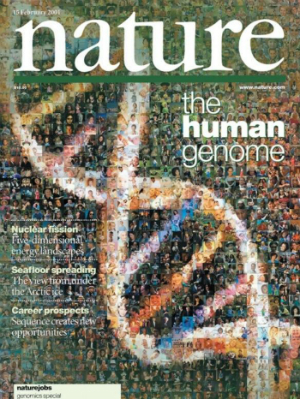
\includegraphics[width=\linewidth, height=0.72\textheight, keepaspectratio]{genomahumanonature.jpeg}
      \par\vspace{0.2em}{\scriptsize \textit{Capa histórica da revista Nature (Fev/2001).}}
    \end{column}
  \end{columns}
\end{frame}

\begin{frame}{Conectoma (2010--2020)}
  \begin{columns}
    \begin{column}{0.52\textwidth}
      \begin{itemize}
        \item \textbf{Human Connectome Project (HCP)}: Mapeamento das conexões neurais estruturais e funcionais do cérebro humano.
        \item Fusão de Ressonância Magnética por Difusão (dMRI), fMRI e teoria dos grafos.
        \item \textbf{Resolução Milimétrica}: Cada voxel ($1\text{ a }2\text{ mm}$) agrupa centenas de milhares de axônios.
        \item Mapeia os grandes feixes de substância branca e hubs de conectividade global.
      \end{itemize}
    \end{column}
    \begin{column}{0.46\textwidth}
      \centering
      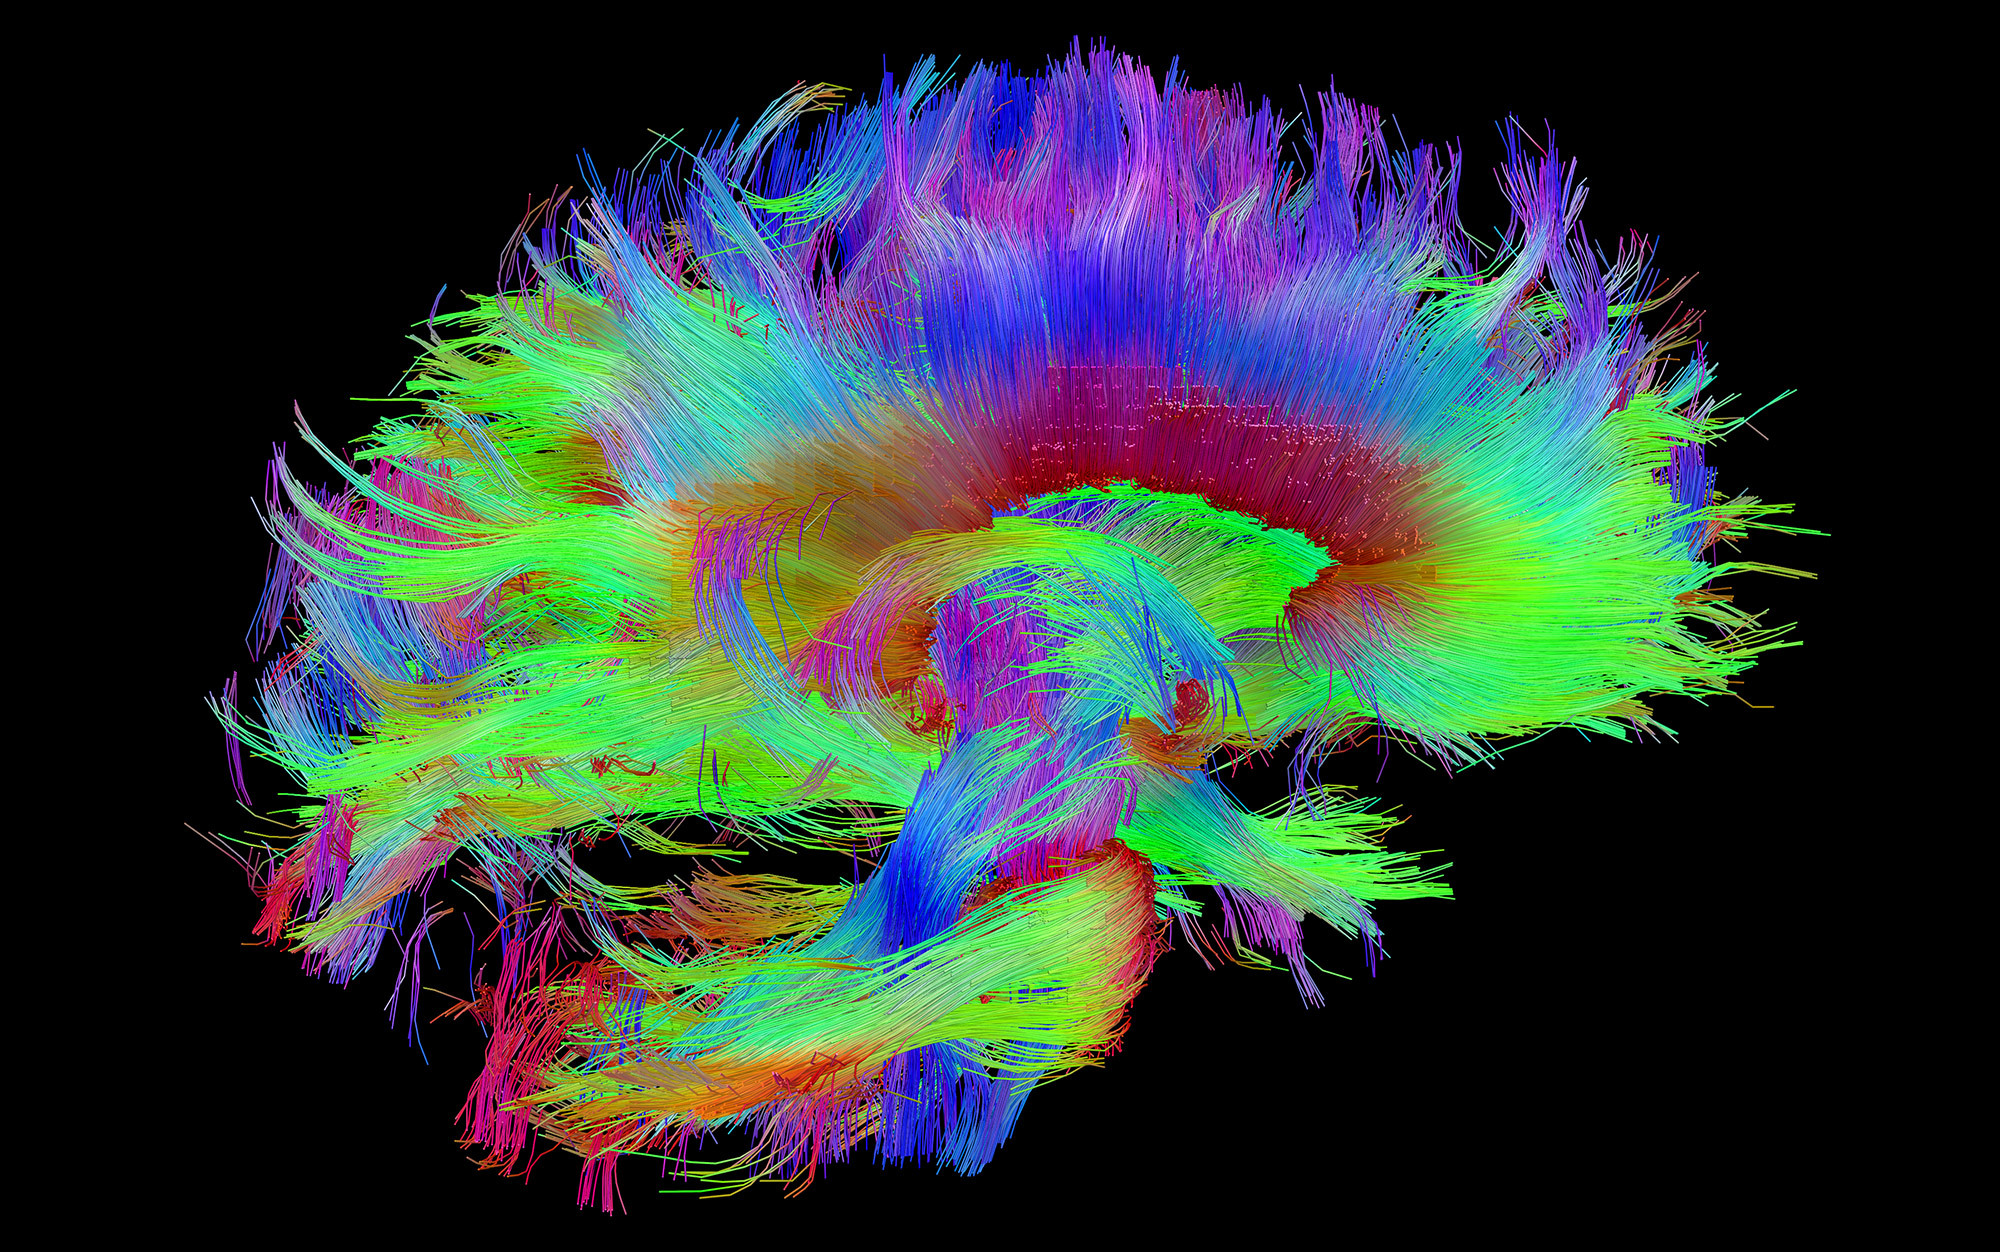
\includegraphics[width=\linewidth, height=0.72\textheight, keepaspectratio]{conectome.jpeg}
      \par\vspace{0.2em}{\scriptsize \textit{Tratografia por difusão (dMRI) e macro-conectoma cerebral.}}
    \end{column}
  \end{columns}
\end{frame}

\begin{frame}{Micro-Conectoma (2024--2026)}
  \begin{columns}
    \begin{column}{0.50\textwidth}
      \begin{block}{O Salto da Escala Nanométrica (\textit{Science}, 2024)}
        Pesquisadores de \textbf{Harvard} e \textbf{Google Research} reconstruíram $1\text{ mm}^3$ de córtex temporal humano em resolução sináptica:
        \begin{itemize}
          \item \textbf{Amostra}: $1\text{ mm}^3$ (metade de um grão de arroz!).
          \item \textbf{Volume de Dados}: \textbf{1,4 Petabytes} (1.400 Terabytes) gerados por microscopia eletrônica serial.
          \item \textbf{Complexidade}: 57.000 células e \textbf{150 milhões de sinapses} mapeadas.
        \end{itemize}
      \end{block}
    \end{column}
    \begin{column}{0.48\textwidth}
      \begin{alertblock}{O Papel da Ciência de Dados e IA}
        A reconstrução manual levaria séculos. Redes neurais de visão computacional da Google segmentaram automaticamente os petabytes de voxels.
      \end{alertblock}
      \begin{exampleblock}{Conectoma Populacional (UK Biobank)}
        Mais de \textbf{100.000 cérebros} escaneados, integrando conectomas a dados genômicos e clínicos em larga escala.
      \end{exampleblock}
    \end{column}
  \end{columns}
\end{frame}


\begin{frame}{GPUs e NVIDIA (1999--2026)}
  \begin{columns}
    \begin{column}{0.53\textwidth}
      \begin{itemize}
        \item \textbf{1999 (GeForce 256)}: A NVIDIA cunha o termo \textit{GPU} voltada à renderização 3D em jogos.
        \item \textbf{2006 (CUDA)}: Computação de propósito geral em GPUs (\textit{GPGPU}), transformando placas gráficas em motores massivos de álgebra linear.
        \item \textbf{2012 (O Marco AlexNet)}: Treinada em duas GPUs NVIDIA GTX 580, deflagra o renascimento das redes neurais e do \textit{Deep Learning}.
        \item \textbf{2024--2026 (IA e Data Science)}:
          \begin{itemize}
            \item Tensor Cores e chips Blackwell viabilizam LLMs e IA generativa em larga escala.
            \item Bibliotecas como \texttt{cuDF} aceleram pipelines de Pandas e NumPy em até 50$\times$.
          \end{itemize}
      \end{itemize}
    \end{column}
    \begin{column}{0.45\textwidth}
      \centering
      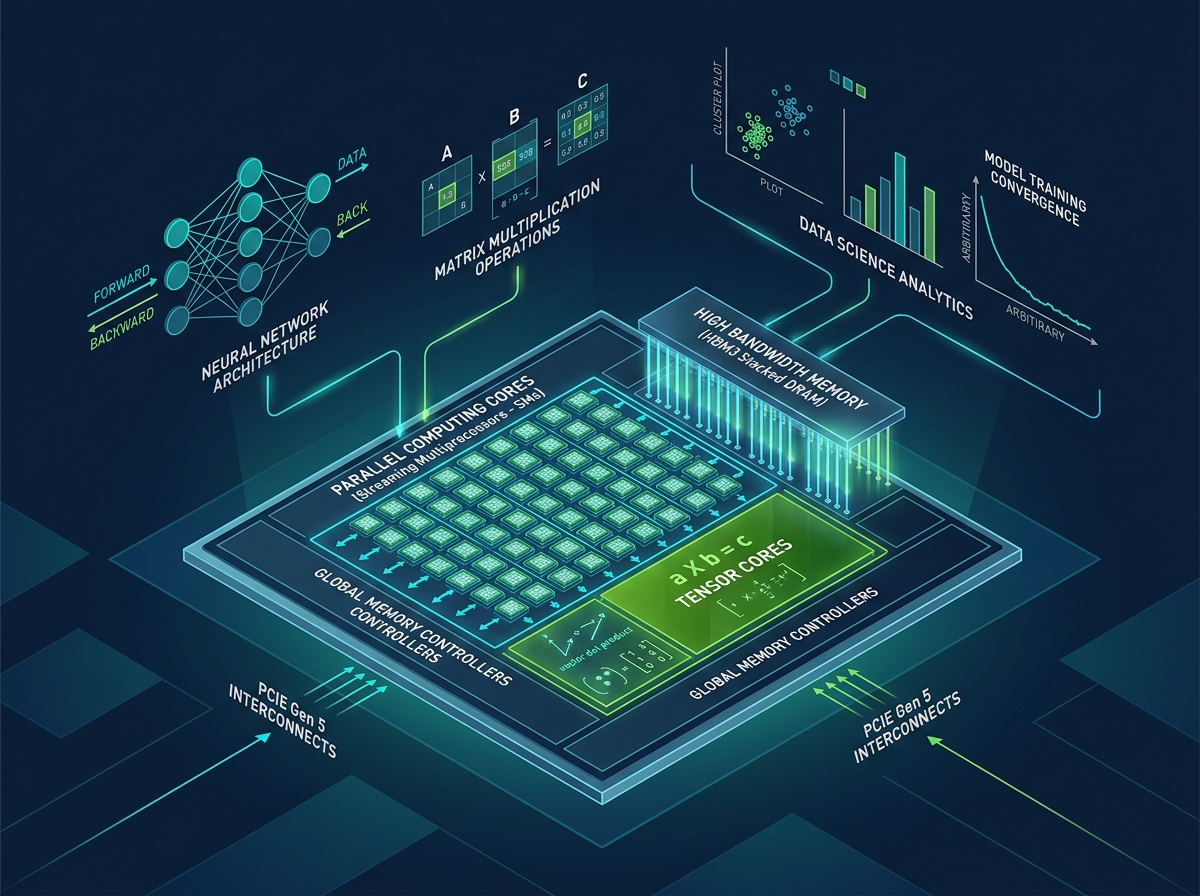
\includegraphics[width=\linewidth, height=0.72\textheight, keepaspectratio]{nvidia_gpu_computing.jpg}
      \par\vspace{0.2em}{\scriptsize \textit{Arquitetura paralela de GPUs, Tensor Cores e aceleração de Ciência de Dados.}}
    \end{column}
  \end{columns}
\end{frame}

% ----------------------------------------------------
\section{O Ciclo de Vida da Ciência de Dados e 2026}
% ----------------------------------------------------

\begin{frame}{O Ciclo de Vida dos Dados (Framework OSEMN)}
  \begin{columns}
    \begin{column}{0.52\textwidth}
      \begin{enumerate}
        \item \textbf{Obtain (Obter)}: Aquisição de bases, sensores, APIs.
        \item \textbf{Scrub (Limpar)}: Tratamento de valores nulos, parsing.
        \item \textbf{Explore (Explorar)}: Análise exploratória de dados (EDA).
        \item \textbf{Model (Modelar)}: Regressão, classificação, clustering.
        \item \textbf{iNterpret (Interpretar)}: Comunicação e tomada de decisão.
      \end{enumerate}
    \end{column}
    \begin{column}{0.46\textwidth}
      \centering
      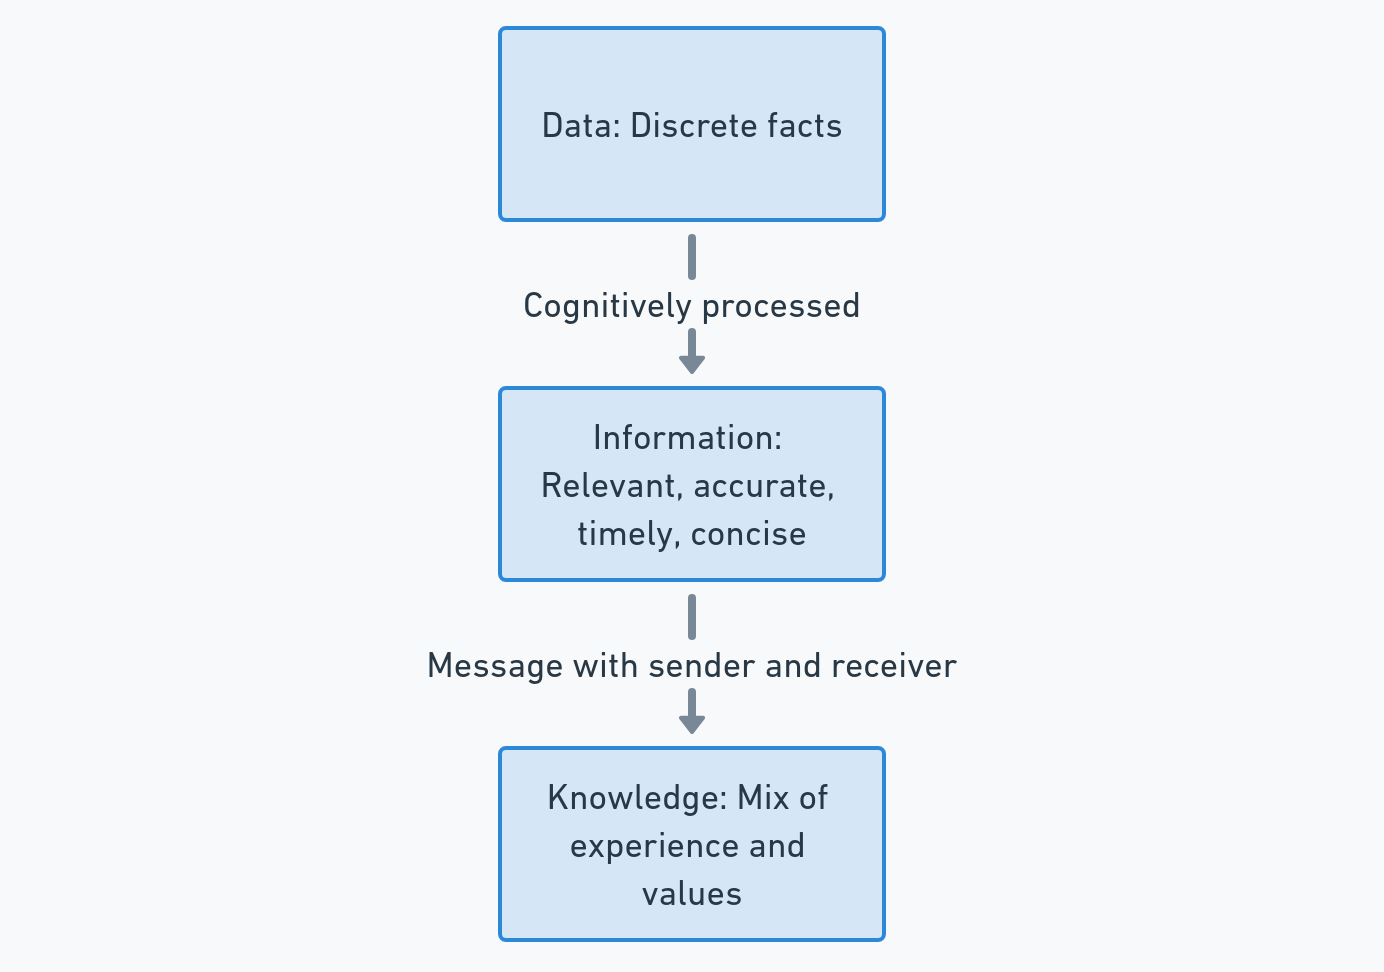
\includegraphics[width=\linewidth, height=0.72\textheight, keepaspectratio]{esquemadata.png}
      \par\vspace{0.2em}{\scriptsize \textit{Esquema do fluxo e ciclo de vida dos dados.}}
    \end{column}
  \end{columns}
\end{frame}

\begin{frame}{A Ciência de Dados em 2026}
  \begin{itemize}
    \item \textbf{Da Escassez ao Dilúvio}: O gargalo contemporâneo não é obter dados, mas destilar sinal a partir do ruído.
    \item \textbf{A Era da IA Generativa e LLMs}: Modelos de fundação atuam como copilotos analíticos, automatizando código básico e acelerando a exploração.
    \item \textbf{Ética e Governança}: Privacidade, LGPD/GDPR, viés algorítmico e auditoria de modelos clínicos na saúde.
    \item \textbf{Reprodutibilidade}: Princípios FAIR (\textit{Findable, Accessible, Interoperable, Reusable}).
  \end{itemize}
  \begin{block}{O Ecossistema Prático deste Curso}
    Python 3.12+, JupyterLab 4, Pandas 2.2+, NumPy 2.x, Matplotlib 3.9+, Seaborn e Scikit-Learn.
  \end{block}
\end{frame}

\begin{frame}{Resumo da Aula 01}
  \begin{itemize}
    \item A necessidade de medir, registrar e analisar dados acompanha a humanidade desde os tabletes de argila e astronomia até o genoma e conectoma moderno.
    \item A Análise Exploratória (EDA) é o alicerce indispensável de qualquer empreendimento científico rigoroso.
    \item \textbf{Atividade Prática}: Acesse o caderno \texttt{Aula01\_Pratica.ipynb} para configurar o ambiente e explorar o catálogo de dados em Python!
  \end{itemize}
\end{frame}

\end{document}
